\documentclass{beamer}
 
\usepackage[utf8]{inputenc}
\usepackage{verbatim}
\usepackage{listings}
\usepackage{hyperref}
\usetheme{Madrid}
 
%Information to be included in the title page:
\title{Compulsory Assignment: Music Box}
\author[Victor, Deivydas, Leila, Biplav]{Victor J. Hansen\inst{1}
\and Deivydas Kazokas\inst{2} \break
\and Leila Mozaffari\inst{3}
\and Biplav Karna\inst{4}
}
\institute{USN Kongsberg}
\date[ES-SHC4300,Feb 2020]{ Software/Hardware co-development of Embedded Systems } 

\begin{document}
 
\frame{\titlepage}
 
\begin{frame}
\frametitle{Overview}
\tableofcontents
\end{frame}

\section{Problem Description}
\begin{frame}
\frametitle{Music Box}
\includegraphics[width=\textwidth, height=0.8\textheight] {../diagram/problem_statement.png}
\end{frame}
 
\subsection{Assumptions}
\begin{frame}
\frametitle{Music Box:Assumptions}
We have assumed below things for design of the music box.
\begin{itemize}
\item Only major notes of octaves 4 and 5 are taken into consideration.
\item The duration of playing note is fixed to 0.5 sec.
\item The user has to start music with '(' and end with ')'.
\item Repeated '(' and ')' will be ignored.
\item Only one music can be stored.
\item The user cannot provide new music when playing.
\item The user can play stored music multiple times.
\end {itemize}
\end{frame}

\section{FSM Block Diagram}
\begin{frame}
\frametitle{FSM Block Diagram}
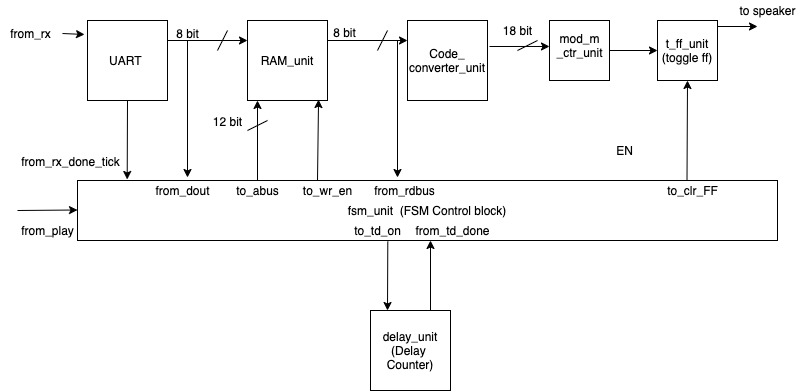
\includegraphics[width=\textwidth,height=0.8\textheight] {../diagram/ccw_music_player-fsm_block_diagram.jpg}
\end{frame}
 
\section{ASMD Diagram}
\begin{frame}
\frametitle{ASMD Diagram}
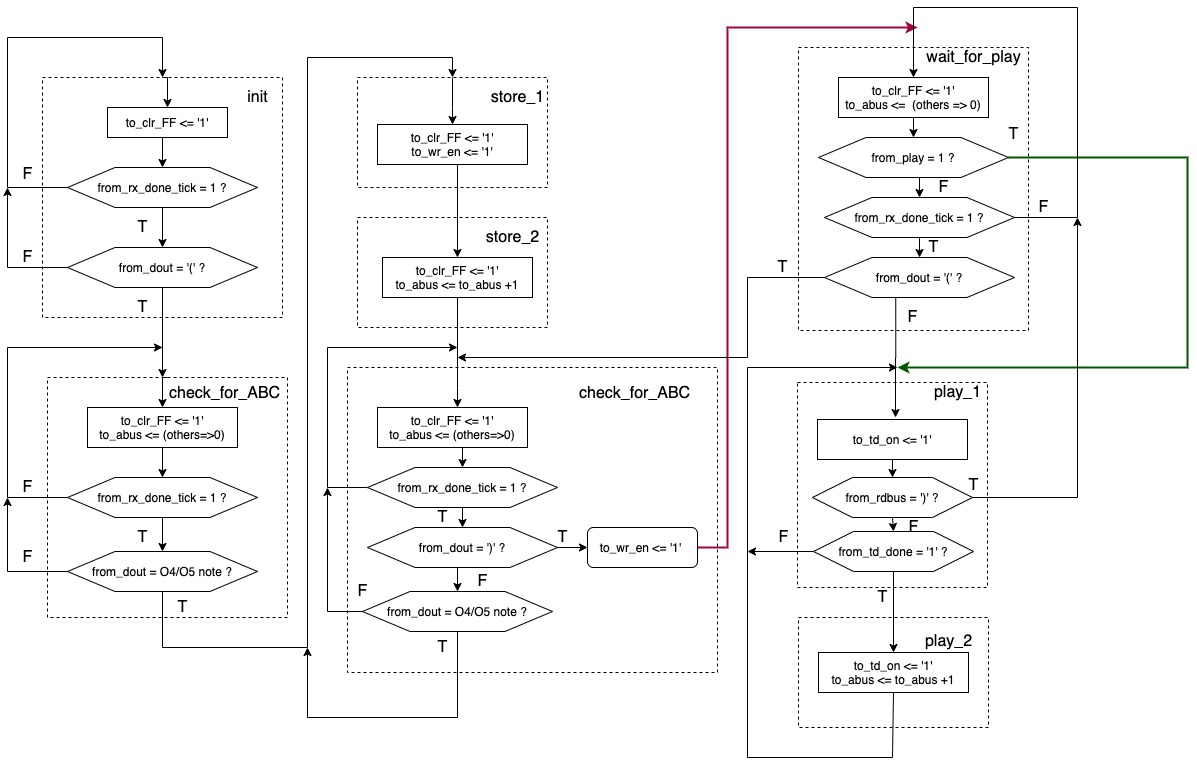
\includegraphics[width=\textwidth,height=0.8\textheight] {../diagram/ccw_music_player-asmd_chart.jpg}
\end{frame}

\section{Code Walkthrough}
\subsection{VHDL Design Walkthrough}
\begin{frame}
\frametitle{VHDL Design Walkthrough}
VHDL Design Walkthrough: Hierarchial 
\begin{itemize}

\item top.vhd
\begin {itemize}
\item uart\_rx.vhd
\begin {itemize}
\item baud\_rate\_generator.vhd
\end {itemize}
\item FSM.vhd
\item RAM.vhd
\item code\_converter.vhd
\item mod\_m\_cntr.vhd
\item t\_ff.vhd
\item timer\_delay.vhd
\end {itemize}
\end {itemize}
\end{frame}

\subsection{Vivado Schematic Diagram}
\begin{frame}
\frametitle{Vivado Schematic Diagram}
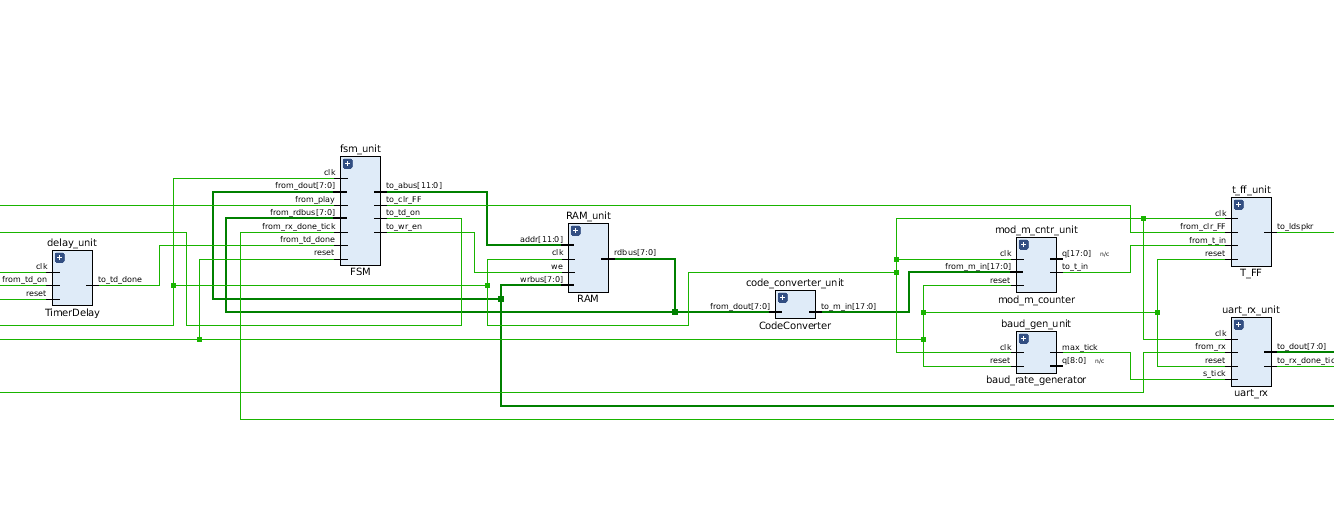
\includegraphics[width=\textwidth, height=0.8\textheight] {../diagram/schematic_diagram.png}
\end{frame}

\subsection{FSM Vhdl Implementation}
\begin{tiny}
\lstinputlisting[language=Vhdl,breaklines=true,title={Snippet of FSM.vhd},frame=shadowbox]{../FSM.vhd}
\end{tiny}

\break

\section{Simulation}
\subsection{Simulation:TestBench Snippet}
\begin{tiny}
\lstinputlisting[language=Vhdl,breaklines=true,title={Snippet of testbench.vhd},frame=shadowbox]{../testbench.vhd}
\end{tiny}

\break

\subsection{Simulation: Vivado Screenshot}
\begin{frame}
\frametitle{Simulation: Vivado Screenshot}
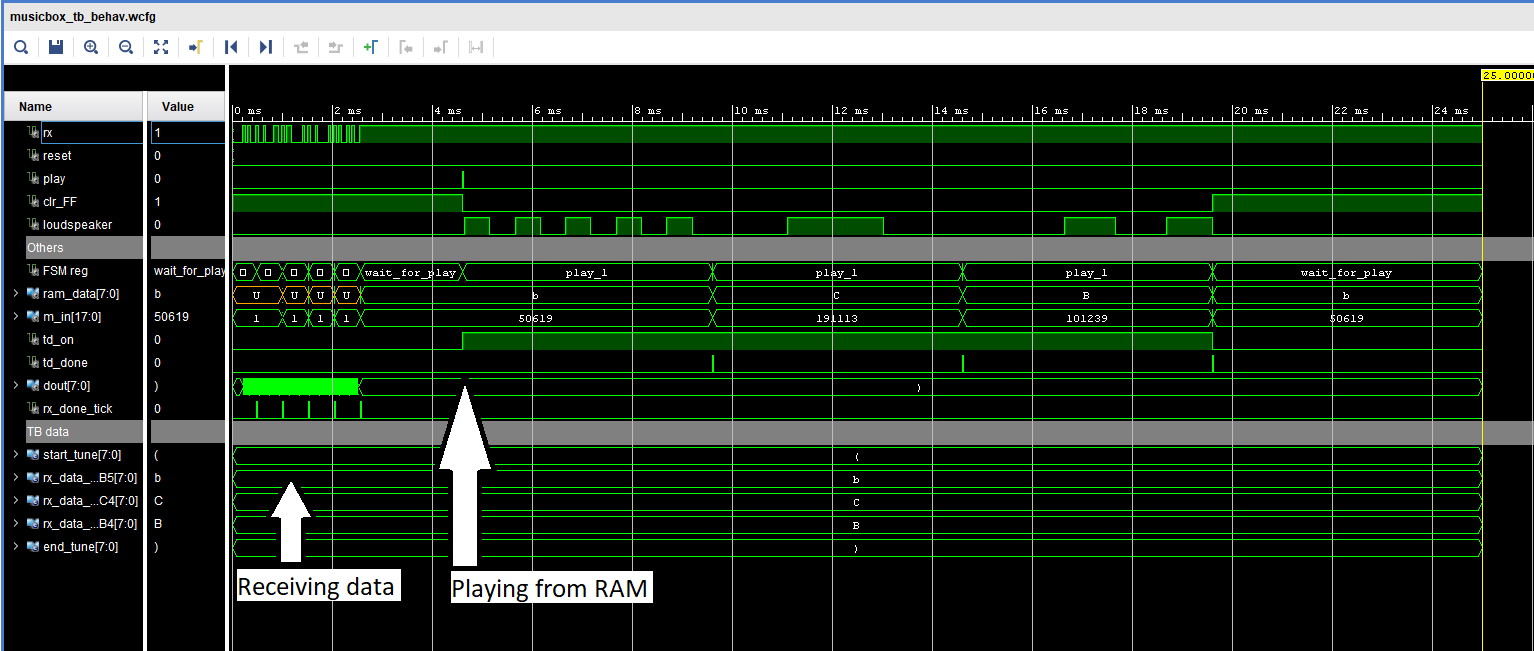
\includegraphics[width=\textwidth,height=0.8\textheight] {../diagram/musicbox_testbench.PNG}
\end{frame}


\section{Video of Project}
\begin{frame}
\frametitle{Video of Project}
A video of the project on basys-3 board is uploaded. Please click the link 
\href{https://drive.google.com/file/d/1TnwBi27fA0xLse6_bEnivC6h0F47zUzk/view?usp=sharing}{\beamerbutton{Watch Full Video} }
\begin{figure}
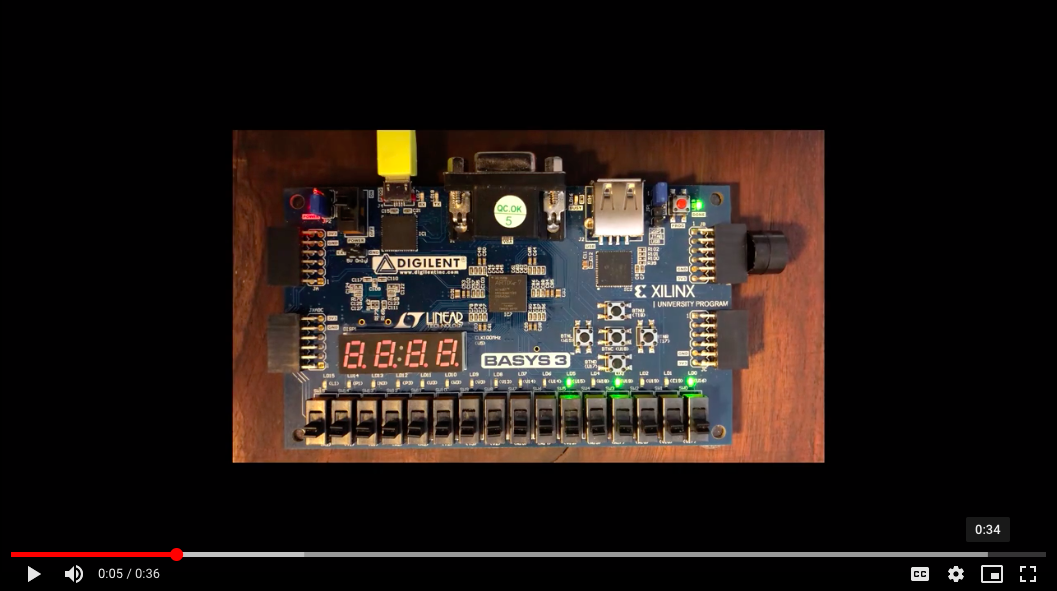
\includegraphics[width=0.7\textwidth,height=0.6\textheight] {../diagram/video_snapshot.png}
\caption{Video Snapshot}
\end{figure}
\end{frame}



\section{Thanks}
\begin{frame}
\frametitle{Thanks}
\centering \Huge
  \emph{Thank You}
\end{frame}

\end{document}
